%Chapter 1

\chapter{绪论}

\section{相关背景与需求}
随着社会发展与技术进步,我国目前越来越重视高效工具的研发。从2000年伊始到2010年互联网普及,再到2020年的现在,个人电子终端的功能已经越来越强大,每个人都需要更新期、更有用的效率工具。近五年,图片标注技术与生成模型都有爆炸式的发展;近两年,视觉问答技术(Visual Question Answering)\upcite{二号文章}、视频标注技术与秒级的图片理解更是让失明群体有了“读懂光芒”的希望,也让图片的理解从学术界或产业界的科研层面有了走向应用、走向市场的可能。

对于看不见的人来说,读懂视野这一技术是他们改善生活质量的工具,画出语言这一技术是他们表达自我的窗口;对更多的普通人群体来说,一个简洁易用的新奇效率工具,更是一种生活方式的改变,让更多的人通过机器的“魔力”,换一种角度来看语言和图片。

\section{技术应用意义与前景}

\subsection{研究意义}
图像-语义的双向翻译在目前已经有了很大的需求面。
最基本的就是,图像作为视觉信号,无法被视觉失能人群感知,可以将语义转化为听觉信号,方便视觉失能人群感知世界。更进一步,对于大量的图像信号,靠肉眼处理起来需要很大的人力成本,如果使用图像标注技术,则可以从图像中提取重要信息,对语义信息进一步处理,形成简报构成参考,辅助决策。

语义的图像化更是意义非凡。基础地说,同样面对失能人群,没有视觉的人通过这一系统也有了“创作”的能力,将他们的思想从肉体的局限中有限地拓宽了出口;或者说,即使是有视觉能力的人,如果不擅长绘画,也可以通过这一技术直接表达自己思想中的画面。更进一步地说,想象力弱是很多成年人能力的局限,而一个语义向图像的转化,则可以使得一个人的表述清晰、直观地呈现在他人的视野里,可以促进交流;而表述之人也可以根据可视化的表达,发现自己表达中的问题,及时予以修正,而这是我们生活中每个人都需要的。

可以说,生成图像不仅仅是作为观赏,它可以切真实际地改变我们的生活方式。

\subsection{研究前景}
现在并没有简单易用的商业系统,可以提供语义与图像互译的简便功能,大部分系统都只能作为技术的样品,做单向的翻译工作,目前主要在各大展览会上起到展示企业技术实力之用。对于常常需要与图片、交流打交道的人来说,这样一套系统对工作效率提高很多;广泛地,对于任何一个人,这类系统都可以改变他的生活方式。

\section{相关工作}

\subsection{循环神经网络}
\subsubsection{朴素神经网络}
神经网络(Neural Networks)是近年比较流行的概念。在2006年Hiinton\upcite{hinton2006reducing}提出深度学习概念后,成为了优化算法表现性能的一大利器。

神经网络的基本结构就是由神经元构成的网络,每个神经元结构如图~\ref{fig:nnc}所示,输入输出关系如式\eqref{eq:nn}表述结果。
\begin{equation}
    \label{eq:nn}
    f( \sum\limits_{i=1}^{m} w_i x_i + b ) 
\end{equation}

对于第$j$层的每一个神经元,它会对上一层的每一个神经元输入的$x_i$赋予权重$w_i$,计算出输出结果,即如式\eqref{eq:nnj}所示,其中n是每一层的神经元个数,由输入神经元个数决定。
\begin{equation}
    \label{eq:nnj}
    x_k^j = \sum\limits_{i=1}^{n} w_ik x_ik, k\in \left[1,n\right]
\end{equation}

\begin{figure}[b]
    \centering
    \begin{minipage}[t]{0.4\linewidth}
        \centering
        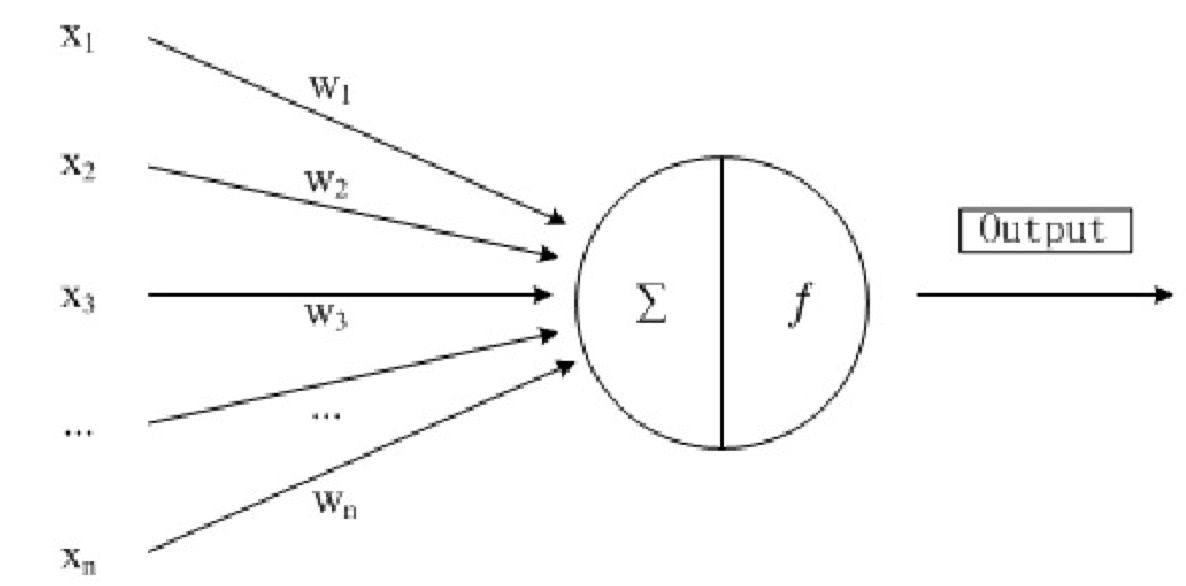
\includegraphics[width=0.9\textwidth]
        {figures/nnc.png}\\
        \caption{神经网络神经元}
        \label{fig:nnc}
    \end{minipage}
    \begin{minipage}[t]{0.5\linewidth}
        \centering
        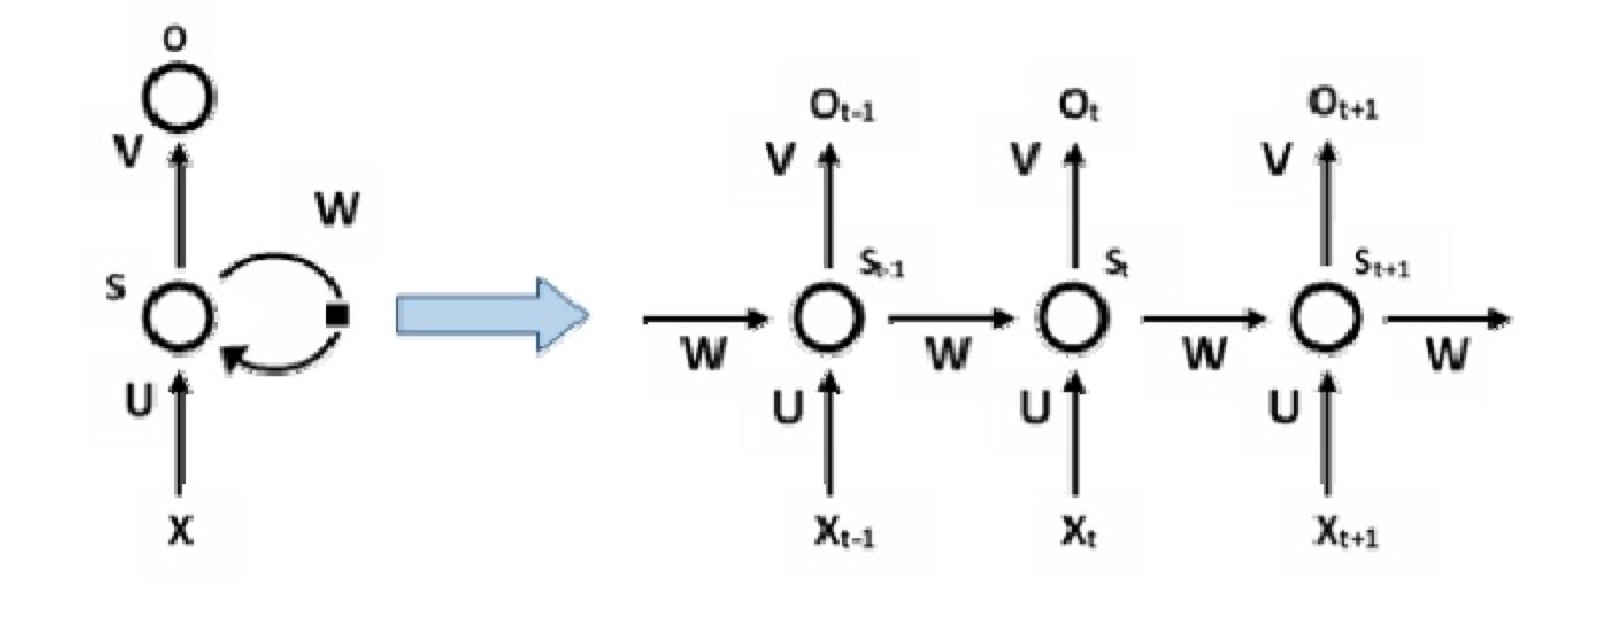
\includegraphics[width=0.9\textwidth]
        {figures/rnnc.png}\\
        \caption{循环神经网络神经元}
        \label{fig:rnnc}
    \end{minipage}
\end{figure}

\subsubsection{循环神经网络}
循环神经网络(Recurrent Neural Networks, RNN)被广泛地运用在图像处理和自然语言处理上。与一般的神经网络相同,它也有前馈层和反馈层,但是它在一般的神经网络基础上增加了基于时序的循环机制。在一般的神经网络中,神经元之间相互独立,但是现实中的信息往往互相关联。所以,循环神经网络的特点像人一样有记忆的能力它的输出不仅依靠当前输入,也依靠历史的输出。在一定程度上,它更能反应真实的情况。

RNN神经元的结构与BP神经网络神经元有些许不同。如图~\ref{fig:rnnc}所示,任一隐藏层中神经元的输出信息依靠当前时刻的输入信息和前序时序的输出信息决定,同时当前时序的输出信息也会作为下一个神经元的输入。这样的神经网络构建了神经元之间的联系,让数据有了更为有效的依赖关系,优化了信息利用的效率。

\subsubsection{长短期记忆}
长短期记忆(Long Short Term Memory, LSTM)作为循环神经网络的一个分支变种,由Hochereiter和Schmidhuber在1997首先提出。在循环神经网络中,一个明显的问题就是参考的上文信息距离当前神经元很远时,就难以参考,影响会变得很小,原因在于梯度消失和梯度爆炸问题。LSTM可以保留重要信息,可以让距离比较远的重要文本对当前神经元产生比较大的影响,可以一定程度优化上下文分析的表现。

\subsection{对抗生成网络}
\subsubsection{背景介绍}
对抗生成网络(Generative Adversarial Networks, GAN)由Goodfellow et al.在2014年首次提出\upcite{goodfellow2014generative}。目前,它已经发展成了生成神经网络最大的热点,其研究得到了长足的发展。短短几年之内,已经有了一百余种GAN网络的衍生模型,其应用范围囊括了包括自然语言、图像处理、计算机视觉在内的各个领域。

在提出GANs模型之前,也有其他的生成式模型存在。生成方法、判别方法分别时机器学习的两大分支方向,而生成式模型则是用生成方法来生成样本的一类模型。有一类生成式模型是从人类理解角度进行设计的,比如说最大似然估计法、近似法\upcite{kingma2013auto,rezende2014stochastic}与马尔可夫链法\upcite{hinton1984boltzmann, ackley1985learning, hinton2006reducing}等,这一类方法对于机器来说各有限制。最大似然估计法的参数更新直接受限于数据样本,数据样本不够丰富会限制生成模型的结果;近似法的目标函数太过复杂,算法只能逼近目标函数下界;马尔可夫链法的缺点便是复杂度过高。从机器理解角度设计的算法一般不直接进行拟合或者估计,而是通过采样数据样本调整模型,一般这种方法人类无法直接理解,但是生成样本是人类可以理解的。

\subsubsection{基本原理}
GANs的基本结构即由一个生成生成模型$G$和一个判别模型$D$组成。生成模型$G$的目的是尽可最小化生成与真实训练样和生成样本的区别,而判别模型$D$的目的则是尽可能最大化地找出真实样本和生成样本之间的区别。

通过多轮迭代生成模型$G$和判别模型$D$的对抗,可以使两个模型都达到上述的目标效果。当训练判别模型$D$的时候,希望输入真实样本$x$可以使判别器对其的判断$D(x)$尽量趋于1,而生成样本$G(x)$通过判别器$D$的时候可以使得$D(G(x))$尽量趋于0。在训练生成模型$G$的时候,输入噪声$z$,希望生成的生成样本通过判别器$D$的时候尽量使得$D(G(z))$趋于0。

可以用简单的数学变换得到公式\eqref{eq:1.1},来描述训练过程。
\begin{equation}
    \label{eq:1.1}
    \min_{G}\max_{D} V_{G,D} = \mathbb{E}_{x \sim P_{data}(x)}[\lg D(x)] + \mathbb{E}_{z \sim P_{G}(z)}[\lg (1-D(G(z)))]
\end{equation}
其中$P_{data}(x)$为真实图片集的分布。

当多轮博弈过后,极大极小问题达到最优解,即纳什均衡,当且仅当$P_z = P_{data}$时\upcite{goodfellow2014generative}。这时$\mathbb{E} D(G(z))$趋于$\frac{1}{2}$,即相当于只能随机猜测0与1,而生成模型$G$学会了真实样本的特性。

相对于传统的生成模型,我们可以发现GANs模型并不需要使用马尔可夫链,学习过程不需要近似推理,也不需要预先训练,自由度比较高,可以利用反向传播计算梯度,很好地利用了分段线性单元的优势,而可以回避近似计算的困难概率问题。

\subsection{自然语言处理}
\subsubsection{背景介绍}
自然语言处理(Natural Language Processing, NLP)是指计算机对自然语言的处理算法。所谓自然语言,就是说人类在社会文明发展过程中为了交流而逐渐发展出的语言,例如中文、英文、日文,甚至包括手语,都是自然语言。因为自然语言之间的关系远远不是函数映射那么简单的事,所以这个领域经历很长的发展历程才到了今天相对成熟的地步。

自然语言处理的发展历程大致分了三个阶段。第一个阶段是上个世纪后半叶,
在二战之后洛克菲勒仅仅会的瓦伦·威佛等人在展望计算机技术的未来应用时,认为计算机可以用不同语言之间的简单词汇替换来完成翻译工作。在现在国际化知识丰富的我们来看,显然可以看出这种方法是行不通的,但是上世纪后期,
大量学者耗费人力物力,建立语言之间的词典,为每一个词汇做了映射,以实现计算机翻译。但是翻译结果并不理想,教训便是自然语言的理解需要考虑上下文关系。第二阶段是世纪之交的二十年。计算机技术迅猛发展,学者开始发现仅靠统计和替换无法完成翻译工作,而且神经网络也初步成熟,人工智能再次登上时代的焦点。例如,2005年,Pradhan\upcite{pradhan2005support}提出了语义角色解析的机器学习算法,使用SVM技术扩展了前人的工作\upcite{surdeanu2003using,gildea2002necessity},改进了数据的泛化功能。

第三阶段是近十年,大数据的积累帮助了自然语言处理的语料库丰富,促进了算法表现的提升;另一方面,音视频处理技术中深度学习的应用更为成熟了。其应用例如:2016年,Y Yao et al.\upcite{yao2016bi}提出了一种基于长短期记忆的中文分词方法,突破了上下文窗口大小限制,可以保存前文的重要信息;2015年Jie Zhou et al.\upcite{zhou2015end}提出了不使用解析的端到端SRL学习系统来分析语义,使用双向RNN,只使用文本作为输入功能,不使用语法知识。

\subsubsection{自然语言应用例子:IBM Watson}
2011年,在美国的一档综艺节目中,IBM公司云服务器bluemix平台上的Watson板块NLP技术相关产品大放异彩,当时因出色的对话表现爆红。

在IBM bluemix云平台上的Watson板块,有多语言对应的多种NLP相关应用,包括语音识别、语音生成等,经过实际试用,发现目前制作水平比较完善,但是中文包的翻译效果比较差。经过调研发现,中文的翻译训练语料库主要是使用专业文件书籍构成,导致语言不够丰富。这也给了我们一个教训,在实际NLP训练中,一定要使用比较丰富、贴近日常生活的语料库。

本文设计以英语为基础,使用了完整、丰富的MSCOCO-2014数据集。有八万多张图片作为训练集,另有四万多张图片作为测试集,且均带有相应的语义标注。这样完整的数据集更贴近一般语言环境,可以得到更好的训练效果。

\subsubsection{基础依赖包}
目前,常用的NLP算法在python、JAVA等语言中里面都有依赖包可以使用。

在我使用的python语言3.7版本中,可以使用依赖包nltk(Natural Language Toolkit)\upcite{nltk},这个包实现了超过五十种自然语言处理的基本算法,可以进行分词、语义角色解析等。

\section{本文工作目标}

\subsection{设计大纲构思}
本次设计需要实现如下功能,并达到要求:
\begin{enumerate}[fullwidth,itemindent=2em,label=\arabic*.]
    %\setlength{\parindent}{4em}
    \item 实现图像生成语义算法,并达到可用的效果;
    \item 实现语义生成图像算法,并且图像对一般人清晰可识别;
    \item 形成一个有机统一的系统,功能简洁易用。
\end{enumerate}

\subsection{本文篇章结构}

本文共分为五个章节。

第一章,介绍了研究的背景,并通过阅读文献,整理了相关的工作,从中找出比较适合于本设计的工作,并加以总结。

第二章,详细介绍了本设计所使用技术的详情,并说明了选取技术原因。

第三章,设计了实验的方案,通过一些前人制作好的开源项目,加以修改、总结,设计系统。

第四章,详细记述了实验的结果,并通过测评手段进行测评,分析了实验结果。

第五章,阐述了设计的意义,并且展望了未来系统进一步扩展迭代的方向,指明了系统的局限性。

\section{本章小结}
本章介绍了设计相关领域的需求背景,也全面地介绍了这一设计的意义与前景。接下来介绍了涉及到的相关技术发展现状和相关领域的工作,也说明了其中最适合于本设计的技术及其原因。最后说明了本设计的基本要求和构思,另外设计了篇章结构,也设定了工作的目标。